\section{直方图分析}

第一个测试是加密、解密和原始图像的直方图分析。 
在这里,各个图像的图像直方图代表了加密图像和原始图像之间的巨大差异,但它们是相同的。 
通过对测试图像的直方图和加密后的直方图的评价,可以观察到加密后的图像在直方图的整个区间内是均匀分布的。 
因此,覆盖了原始图像的分布规律。 因此,有效地实施了加密(参见图\ref{fig:4.3})。

\begin{figure}[ht]
    \begin{center}
        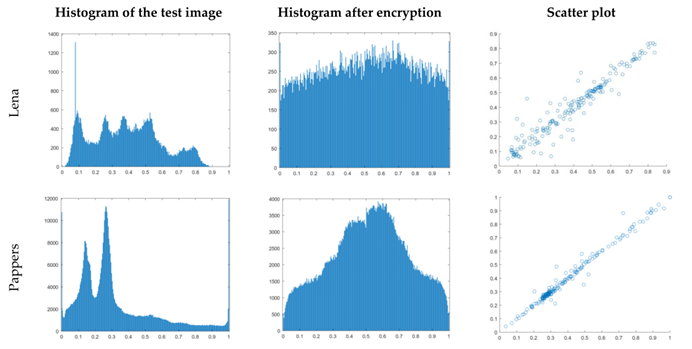
\includegraphics[width=\textwidth]{figure/p5.png}\\
        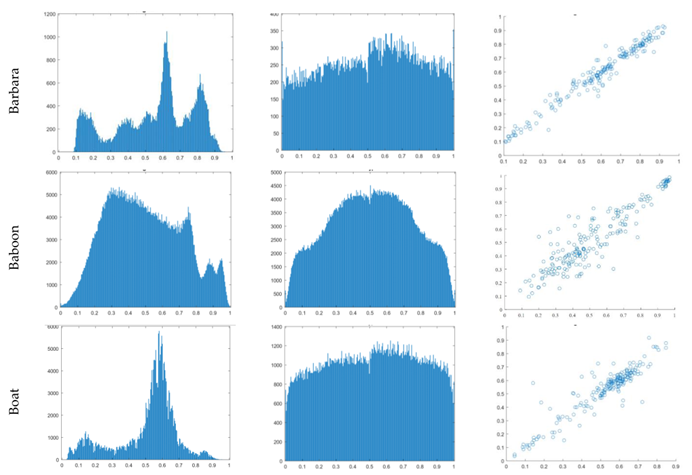
\includegraphics[width=\textwidth]{figure/p6.png}\\
    \end{center}
    \caption{原始 Lena 图像的直方图分析 \label{fig:4.3}}
\end{figure}